\chapter{TMS-1000}

\newpage

\section{Geschichte}

W{\"a}hrend Intel es erstmals schaffte alle Bausteine eines Prozessors auf einem Mikrochip zu vereinigen, implementierte Texas Instruments parallel zus{\"a}tzlich Peripherie auf dem Chip und schuf so den ersten Mikrocontroller, welcher auch System-on-a-Chip genannt wurde. \\
Texas Instruments wurde 1951 von Cecil Howard Green, Jon Erik Jonsson, Eugene McDermott und Henry Bates Peacock gegr{\"u}ndet. Das Unternehmen war unter anderem f{\"u}r den ersten integrierten Schaltkreis bekannt. Die Konstruktion eines System-on-a-Chip gelang erstmal den Ingeneuren Gary Boone und Michael Cochran mit dem Controller TMS-1000 im Jahre 1971. Texas Instruments stellte verschiedene Versionen des TMS-1000 her, die in Gr{\"o}{\ss}e des ROM und RAM Speichers variierten. Anfangs verwendete die Firma die Controller nur in eigenen Produkten, vor allem Taschenrechner, wie der SR-16, welcher 1972 auf den Markt kam. Die Firma ist aus diesem Grund und aufgrund der zahlreichen Nachfolger f{\"u}r ihre Taschenrechner bekannt. \\
Erst 3 Jahre nach der Erfindung, also 1974, war der TMS-1000 auf dem freien Markt erh{\"a}ltlich. Dies hatte jedoch zur Folge, dass der Markt durch Intel mit ihren Mikroprozessoren schon zum gro{\ss}en Teil eingenommen war. Trotzdem hatte der Controller aufgrund seines extrem niedrigen Preises, 2\$ pro St{\"u}ck, gro{\ss}en Erfolg auf dem Markt. Der TMS-1000 half dadurch die moderne Elektronik f{\"u}r jedermann zug{\"a}ngig zu machen. Der Controller fand nicht nur in Taschenrechnern Verwendung, sondern auch in ersten Handheld-Ger{\"a}ten, Jukeboxen, T{\"u}rklingeln, Uhren und vielen mehr. Bis zum heutigen Tag wurden ca. 100 Millionen Controller verkauft.

\section{Mikrocontroller}
\subsection{Aufbau}
Mikrocontroller werden nicht zu Unrecht System-on-a-chip genannt und der Aufbau eines Controllers kann daher sehr gut mit den Bestandsteilen eines Computers verglichen werden. Im folgenden werden die Komponenten eines Computers und die Bestandteile eines Mikrocontrollers vergliechen. Au{\ss}erdem wird die Aufgabe der einzelnen Bauteile des Controllers beschrieben. 

\newpage
\begin{tabular}{| l | l | l |}
	PC & Mikrocontroller & Aufgabe \\ \hline
	Prozessor & CPU & Der Prozessor f{\"u}hrt die aritmethische und \\
	 & & logische Operationen aus \\ \hline
	Arbeitsspeicher & RAM & RAM ist ein tempor{\"a}rer Speicher f{\"u}r Variablen. \\
	& & Verliert den Speicherinhalt nach dem Entfernen \\
	& & der Betriebsspannung \\ \hline
	Festspeicher & ROM & Enth{\"a}lt das Programm \\ \hline
	Takt & Takt & Gibt die Geschwindigkeit der Befehls- \\
	& & folge an \\ \hline
	Peripherie & I/O-Ports & Der Controller enth{\"a}lt einfach Ein- \\
	& & und Ausg{\"a}nge f{\"u}r beispielsweise \\
	& & LEDs, Displays und Schalter \\ \hline
	
\end{tabular}

\subsection{Abgrenzung zu Mikroprozessoren}

Oftmals ist es schwierig eine klare Grenze zwischen Mikroprozessoren und Mikrocontrollern zu ziehen. Das liegt vor allem daran, dass nach einiger Zeit mei{\ss} Mikrocontroller-Varianten von neuen Mikroprozessor-Architekturen erschienen sind. Die haupst{\"a}chliche Abgrenzung erfolgt durch die Austattung der Zusatzmodule des Chips. W{\"a}hrend ein Mikrocontroller einen Prozessor inklusive Bausteine wie Speicher, In- und Outputs, Timer, usw., konzentriert sich ein Mikroprozessor auf seine eigentliche Hauptaufgabe, die Rechengeschwindigkeit. Durch den gesparten Platz auf dem Chip wird diese wesentlich erh{\"o}ht.

\subsection{Architekturen}

Viele der verbauten Mikrocontrollern verwendet 8-Bit-Prozessoren, deren Architektur auf die 1970er Jahre zur{\"u}ckzuf{\"u}hren ist. Allerdings gibt es auch 4-, 16- und 32-Bit Mikrocontroller. Die ersten Controller die gebaut wurden waren dabei 4-Bit-Controller und sind deswegen heutzutage noch stark vertreten. Den gr{\"o}{\ss}ten Marktanteil haben mittlerweile die 32-Bit-Controller da die meisten heutigen Mikrocontroller auf Prozessorkernen basieren, von denen 8- und 16-Bit Prozessoren fast nicht mehr hergestellt werden.

\section{TMS-1000}

\subsection{Allgemeine Daten}

Der TMS-1000 geh{\"o}rt zur Familie der 4-Bit Mikrocontroller. Die Gr{\"o}{\ss}e des ROMs des Controllers betr{\"a}gt 8.192 Bits, w{\"a}hrend die des RAMs 256 Bits betr{\"a}gt. Die maximale Spannung, welche an der Clock und sowohl an den Eingang- und Ausgang-Pins angelegt werden darf, bemisst sich auf 20 Volt. Durch die intern verbauten Oszilliatoren kann der Controller einen Takt von bis zu 0,4 MHz erreichen. Jede Instruktion ben{\"o}tigt 6 Oszilliatoren-Zyklen um vollst{\"a}ndig ausgef{\"u}hrt zu werden. Insgesamt verf{\"u}gt der TMS-1000 {\"u}ber 43 Basisinstruktionen, 12 fixierte und 31 programmierbare. 

\subsection{Pins}

Der TMS-1000 verf{\"u}gt {\"u}ber insgesamt 28 Pins. 

\begin{figure}[!htb]
	\centering
		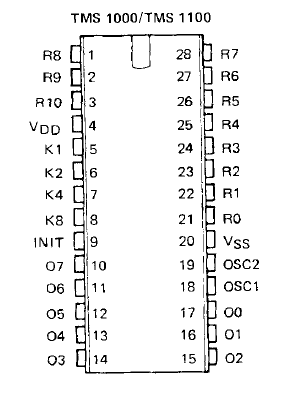
\includegraphics[width=0.40\textwidth]{figures/pins_TMS1000.PNG}
	\caption{Skizze der Pins}
	\label{fig:pins_TMS1000}
\end{figure}

\newpage

\begin{tabular}{| l | l | l |}
Bezeichnung & Anzahl & Aufgabe \\ \hline
R-Output & 11 & F{\"u}r die Ausgabe von Kontroll-Daten zust{\"a}ndig \\ \hline
O-Output & 8 & Gibt den Inhalt des Akkumulators und das Status-Logic-Bit aus \\ \hline
Oszillatoren & 2 & Zust{\"a}ndig f{\"u}r den Takt des Controllers \\ \hline
Power-Supply & 2 & Versorgt den Controller mit Spannung \\ \hline
K-Input & 4 & Eingang f{\"u}r 4-Bits zur Verwendung im Programm \\ \hline
INIT & 1 & Initialisiert oder setzt die Hardware zur{\"u} \\ \hline
\end{tabular}

\subsection{Aufbau \& Funktionsweise}

Der folgende Abschnitt befasst sich mit dem Aufbau und der Funktionsweise der Hardware des Mikrocontrollers TMS-1000. 

\subsubsection{ROM - Read Only Memory}

Der Festspeicher besteht aus 16 Seiten, welche je 64 W{\"o}rter enthalten. Jedes Wort ist dabei 8 Bits gro{\ss}. Es werden 4 verschiedene Register benutzt um den Speicher zu adressieren. \\
\\
Das Page Adress Register(PA): Dieses Register enth{\"a}lt die aktuelle Seitenanzahl, an dem sich das Programm zur Zeit befindet. Das Register ist 4-Bits gro{\ss}, um alle Seiten von 0 bis 15 adressieren zu k{\"o}nnen. \\
Das Page Buffer Register(PB): Das PB-Register wird mit einer neuen Seitenadresse geladen und nach einer erfolgreichen Branch oder Subroutinen-Operation wird die Adresse in das PA-Register geladen. Aus diesem Grund entspricht die Gr{\"o}{\ss}e des Registers der des PA-Registers \\
Das Program Counter Register(PC): Dieses Register enth{\"a}lt das aktuelle Wort der Seite, in dem sich das Programm zur Zeit befindet. Um alle 64 W{\"o}rter adressieren zu k{\"o}nnen enth{\"a}lt das Register 6 Bits. \\
Das Subroutine Return Register(SR): In dem SR-Register wird bei einer Call Operation das aktuelle Wort des Porgramms gespeichert, um bei einer Return Instruktion zum urspr{\"u}nglichen Wort zur{\"u}ckkehren zu k{\"o}nnen. 

\subsubsection{Branching \& Subroutinen}

Branching und Subroutinen sind ein essentieller Teil der im Ablauf eines Mikrocontroller-Programms. Ein Branch ist mit einer herk{\"o}mmlichen if-Abfrage aus einer beliebigen Programmiersprache gleichzusetzen. Der Branch wird erfolgreich ausgef{\"u}hrt, wenn das Status-Logic-Bit gesetzt ist. Das Bit ist zwar standardm{\"a}{\ss}ig gleich 1, kann durch Rechenoperationen, oder Vergleiche durch die Recheneinheit gleich 0 gesetzt werden. Nach einem Instruktionszyklus wird der Zustand wieder zur{\"u}ck gesetzt. Bei erfolgreicher Ausf{\"u}hrung eines Branches wird das PB-Register in das PA-Register geladen. \\
\\
Subroutinen sind sehr {\"a}hnlich zu Branch Instruktionen. Bei einer erfolgreichen Call-Instruktion springt das Programm, an eine andere Adresse im ROM. Bei einer Return-Instruktion kehrt das Programm zu dem urpr{\"u}nglichen Call-Statement zur{\"u}ck. Die Subroutine wird genau wie bei einem Branch nur ausgef{\"u}hrt, wenn das Status-Logic-Bit gesetzt ist. Zus{\"a}tzlich muss jedoch das so genannte Call-Latch gesetzt sein. In diesem Fall wird der Inhalt des PA-Registers mit dem des PB-Registers vertauscht. Die Adresse des PC-Registers wird in dem SR-Register zwischengespeichert. Bei der ReturnInstruktion werden die tempor{\"a}r gespeicherten Adressen wieder in das PA- und PC-Register geladen. Es ist nicht m{\"o}glich eine Call Instruktion innerhalb einer Call Instruktion aufzurufen, ohne dass die korrekte Return-Adresse verlorgen geht.

\subsubsection{RAM - Random Access Memory}

Der RAM-Speicher besteht aus 4 Dateien, welche jede 16 W{\"o}rter enthalten. Jedes Wort ist dabei 4 Bit gro{\ss}. Der Speicher wird durch 2 Register X und Y adressiert. Das X-Register gibt dabei die Datei an, das Y-Register das Wort.\\
Der Input erfolt durch den Write-Multiplexer. Sowohl das Akkumulator Register, als auch die Constant and K Input Logic (CKI) k{\"o}nnen in den Speicher schreiben. Der Read-Bus {\"u}bernimmt den Output des RAMs. Der Bus schreibt die das Wort entweder in den P-Multiplexer oder den N-Multiplexer, welche beide in die Recheneinheit f{\"u}hren. Die Recheneinheit leitet die Daten entweder in das Y oder Akkumulator Register. \\
Dem Programmierer des Controllers steht es frei, wie er sich den Speicher einteilt. Typischerweise werden die ersten 7 W{\"o}rter jeder Seite f{\"u}r als Register verwendet. Der Rest wird durch beispielsweise Pointer, Event Counter oder Flags bef{\"u}llt. Diese sollten sich wenn m{\"o}glich



